\documentclass[11pt]{article}
% Command line: pdflatex -shell-escape compulse.tex
\usepackage{geometry} 
\usepackage{amsmath}
\usepackage{amssymb}
\usepackage{booktabs}
\usepackage{times}
\usepackage{bm}
\usepackage{fixltx2e}
\usepackage[outerbars]{changebar}
\usepackage{graphicx}
\usepackage{epstopdf}
\usepackage{color}
\usepackage{tabularx}
\usepackage{ulem}
%\usepackage{verbatim}
\usepackage{textcomp}
\usepackage{hyperref}
\hypersetup{colorlinks=false,urlcolor=blue,linkcolor=blue}
\usepackage{caption}

\epstopdfsetup{suffix=} % to remove 'eps-to-pdf' suffix from converted images
%\usepackage{todonotes} % use option disable to hide all comments

\usepackage[sort&compress]{natbib}
\bibpunct{[}{]}{,}{n}{,}{,}

%\usepackage[noend]{algpseudocode}

\usepackage{dsfont}
\usepackage{relsize}

%\usepackage{todonotes}

%\graphicspath{{Figure/}}

%changing the Eq. tag to use [] when numbering. use \eqref{label} to reference equations in text.
\makeatletter
  \def\tagform@#1{\maketag@@@{[#1]\@@italiccorr}}
\makeatother

\linespread{1.5}
%\setlength{\parindent}{0in}

% the following command can be used to mark changes made due to reviewers' concerns. Use as \revbox{Rx.y} for reviewer x, concern y.
\newif\ifmarkedup
\markeduptrue

\ifmarkedup
	\newcommand{\revbox}[1]{\marginpar{\framebox{\textcolor{blue}{#1}}}}
\else
	\newcommand{\revbox}[1]{}
	\renewcommand{\textcolor}[1]{}
	\renewcommand{\sout}[1]{}
\fi

%\newcommand{\bop}{$\vert B_1^+ \vert$}
\newcommand{\kt}{$k_\textrm{T}$}
\newcommand{\bmap}{$B_1^+$}
\newcommand{\mytilde}{\raise.17ex\hbox{$\scriptstyle\mathtt{\sim}$}}  % tilde symbol
\mathchardef\mhyphen="2D

\begin{document}

\title{k-Space Domain Parallel Transmit Pulse Design}
\author{Jun Ma$^{1,2}$, Bernhard Gruber$^{3,4}$, Xinqiang Yan$^{1,5}$, and William A. Grissom$^{1,2,5*}$}
\maketitle
\begin{flushleft}
\vspace{-0.5cm}
$^1$Vanderbilt University Institute of Imaging Science, Nashville, TN, United States\\
$^2$Department of Biomedical Engineering, Vanderbilt University, Nashville, TN, United States\\
$^3$A. A. Martinos Center for Biomedical Imaging, Massachusetts General Hospital, Harvard Medical School, Charlestown, MA, United States\\
$^4$Division MR Physics, Center for Medical Physics and Biomedical Engineering, Medical University Vienna, Vienna, Austria\\
$^5$Department of Radiology and Radiological Sciences, Vanderbilt University, Nashville, TN, United States\\    

\par
-------------------------- 

\par
Word Count: Approximately 5500 \\
*Corresponding author: \\
Will Grissom\\
Department of Biomedical Engineering\\
Vanderbilt University\\
5824 Stevenson Center\\
Nashville, TN 37235 USA \\
E-mail: will.grissom@vanderbilt.edu \\
Twitter: @wgrissom

\par Submitted to Magnetic Resonance in Medicine for consideration as a Full Paper.

\par
Acknowledgment: This work was supported by NIH grants R01 EB016695 and U01 EB 025162.

\end{flushleft}
\thispagestyle{plain}

\pagebreak

%%%%%%%%%%%%%%%%%%%%%%% Abstract %%%%%%%%%%%%%%%%%%%%%%%

\section*{\underline{Abstract}} 
{\bf Purpose:}
To accelerate the design of multidimensional parallel transmission pulses. 
\\[1em]
{\bf Methods:}
A k-space domain parallel transmission pulse design algorithm was proposed that
produces a sparse matrix relating a target excitation pattern to the pulses that produce it,
and can be finely parallelized. 
The algorithm was applied in simulations to the design of 3D SPINS pulses for inner volume excitation in the brain at 7 Tesla.
It was characterized in terms of the dependence of computation time, excitation error, and required memory
on algorithm parameters,
and it was compared to the spatial domain pulse design method in terms computation time, excitation error,
Gibbs ringing, and ability to compensate off-resonance.
\\[1em]
{\bf Results:}
The proposed algorithm achieved approximately 90\% faster pulse design compared to 
an iterative spatial domain method, with the same number of parallel threads,
with the tradeoff of increased excitation error and RMS RF amplitude. 
It reduced the memory required to store the design matrix by 98\% compared to a full matrix solution.
Even with a coarse design grid, the algorithm produced patterns that were free of Gibbs ringing.
It was similarly sensitive to k-space undersampling as the spatial domain method,
and was similarly capable of compensating for off-resonance.
\\[1em]
{\bf Conclusion:}
The proposed k-space domain algorithm accelerates and finely parallelizes parallel transmission pulse design,
with a modest tradeoff of excitation error and RMS RF amplitude.
\\[1em]
{\bf \noindent Key words:} Parallel Transmission; RF pulses; Ultra-high field MRI; RF pulse design; Selective excitation.

\pagebreak

%%%%%%%%%%%%%%%%%%%%%%% Main Text %%%%%%%%%%%%%%%%%%%%%%%

\section* {Introduction}

\par Multidimensional RF pulses have been widely used in many applications such as reduced field-of-view imaging \cite{rieseberg2002two}, transmit field inhomogeneity correction \cite{saekho2005small}, and susceptibility artifacts correction \cite{stenger2000three}. Parallel transmission (pTx) \cite{katscher2003transmit,zhu2004parallel} further strengthens the multidimensional pulses by providing extra spatial encoding power, shortening pulse duration, and reducing  specific absorption rate (SAR). However, current multidimensional pTx pulse design methods are based on a spatial domain formulation \cite{Grissom:2006:MRM,setsompop2008magnitude} that has prohibitive memory and computational requirements when the number of coils and the number of dimensions both become larger in current designs. 
Particularly, current spatial domain design methods map any given RF pulse $\mathbf{b}$ to its spatial excitation pattern $\mathbf{d}$ with a large system matrix $\mathbf{A}$, as:
\begin{equation*}
	\mathbf{d}=\mathbf{Ab}
\end{equation*}
The size of $\mathbf{A}$ is $N_s$ by $N_cN_t$, where $N_s$ is the number of spatial locations, $N_c$ is the number of coils, and $N_t$ is the number of RF samples. Since $N_s$ becomes unbearably large in designs such as 2D plus spectral and 3D problems, and $N_c$ increases with more advance hardware designs, this $\mathbf{A}$ matrix is typically too large to find the inverse in terms of memory. Therefore, such design problems need to be solved by iterative conjugate-gradient (CG) methods which avoid matrix inversion. However, even if no matrix inversions are performed, the large system matrix may still be memory-inefficient when used in many matrix multiplications over a large number of iterations, making the solving process very slow. Furthermore, the NUFFT-based pulse design methods can also be slow due to all the gridding steps. Although these can be eliminated in NUFFT-based image reconstruction using Toeplitz formulation, in RF pulse design the Toeplitz formulation does not exist since the inner product is over space. 
These slow design methods are especially undesirable when tailored pulses are needed to be designed for each subject during one's examination in the scanner. Typically, the subject-tailored pulse design has to be done within one minute in the pre-scan stage, so that the incorporation of subject-tailored pulses into currently used workflow is practical and desirable.  

\par One application of subject-tailored multidimensional pTx pulses that is of particular interest of this dissertation is the 3D inner volume suppression (IVS) pulses for MR Corticography (MRCoG).MRCoG is a developing imaging technique which aims for submillimeter isotropic resolution whole-cortex and cortex-specific imaging. 
It is a promising technique to enable whole-brain functional and diffusion studies of the columnar and laminar subcortical structures, which are the fundamentals of higher-order brain functions. 
%The current columnar and laminar fMRI methods all use a small field of view in order to achieve sub-millimeter resolution. This does not allow studies to be performed across the whole cerebral cortex. On the other hand, current whole brain fMRI methods typically have spatial resolution greater than 1 mm, which is not sufficient for the studies of columnar and laminar structures. 
MRCoG will use IVS to enable highly accelerated imaging of the cortex, by reducing g-factor and suppressing physiological noise from ventricle CSF. Therefore, subject-tailored IVS pTx pulses are needed, which could be applied before each excitation and readout. Thanks to the high performance gradient system an the 24-channel transmit system of the developing MRCoG scanner, good IVS with 3D selective excitation pulses becomes feasible. However, this IVS pulse design problem is challenging due to its 3D nature and the large number of transmit channels. 

\par Here we propose a k-space-based approach to pTx pulse design that has low memory and computational requirements, and is highly parallelizable. Specifically, we build a sparse system matrix $\mathbf{W}$ that relates the Fourier transform of the spatial domain desired pattern and the desired RF pulse, so that the RF pulse can be instantaneously solved by a sparse matrix multiplication with no matrix inversion or iterative CG method. We advance the work by Katscher et al \cite{katscher2003transmit} by solving the columns of the system matrix in a parallelized fashion. This is done by utilizing the independence between columns of the system matrix which comes from the compactness of sensitivity maps in k-space. In the following text, we will derive the independent solution to each column and show a patch-wise parallelization that allows the control of the size and accuracy of each instance problem. We further accelerate the solution of each instance problem by proposing an efficient method to construct a key matrix needed while maintaining accuracy. Off-resonance correction is also incorporated into this k-space domain design. Then we apply this k-space domain design method to the 3D IVS pulse design problem, and demonstrate its striking acceleration to the computation speed by comparing its performance to the conventional spatial domain design method through simulations. We show how the computation speed and accuracy can be traded off through controlling the parameters of the patch-wise parallelization. We also demonstrate the k-space domain design's ability to accommodate excitation k-space undersampling and correct off-resonance.  

\section*{Theory}

\subsection*{k-space domain parallel-transmit pulse design}
\par Here we describe the derivation of the highly parallelizable k-sapce domain design method. We propose to find a system matrix $\mathbf{W}$ that directly maps a desired excitation pattern in k-space $\mathcal{F}(\mathbf{d})$, which is the Fourier transform of the spatial domain desired pattern $\mathbf{d}$, to the corresponding desired RF pulse $\mathbf{b}$, as:
\begin{equation*}
\mathbf{b}=\mathbf{W}\mathcal{F}(\mathbf{d})
\end{equation*}
$\mathcal{F}(\mathbf{d})$ is the vectorized k-space excitation pattern with length of $N_s$, which is the number of spatial/k-space locations.  $\mathbf{b}$ is the concatenated multi-channel RF samples with length of $N_tN_c$, where $N_t$ and $N_c$ are the numbers of time points and coils, respectively. $\mathbf{W}$ is the $N_tN_c$ by $N_s$ system matrix, which will latter be shown sparse.
Therefore, once the $\mathbf{W}$ matrix is found, the RF design problem can be instantaneously solved by a sparse matrix multiplication, and there is no matrix inversion or iterative CG method needed. Furthermore, in design problems involved iterative procedures, such as the phase updates in magnitude-least-squares pulse designs \cite{setsompop2008magnitude} and the regularization factor updates in power/roughness constrained pulse design, the sparsity of the $\mathbf{W}$ matrix makes the iterative process much more efficient in terms of memory and speed. In the work of Katscher et al \cite{katscher2003transmit}, parallel transmit pulse design was also formulated in the k-space domain. However, in Ref \cite{katscher2003transmit}, the matrix $\mathbf{W}$ was solved as a whole, which required constructing and inverting a large $\mathbf{S}^H\mathbf{S}$ matrix, which will be explained in the following text. Our proposed method finely divides the process of finding $\mathbf{W}$ into many independent instances, which allows the use of parallel computing to largely accelerate the computation. Furthermore, the $\mathbf{S}^H\mathbf{S}$ matrices of different instances are each small, and our proposed method efficiently constructs these matrices, which further accelerates the computation. 

\par We can solve for the columns of the $\mathbf{W}$ matrix independently to each other, based on the key observation that if the desired k-space pattern is a delta function at a given k-space location $\vec{k}_i$ ($1\leq i \leq N_s$), then only the $i$-th column $\mathbf{w}_i$ of $\mathbf{W}$ relates the desired k-space pattern to the desired RF pulse. In this case, the vector $\mathbf{w}_i$ is identical to the desired RF. Therefore, the question of finding the $i$-th column $\mathbf{w}_i$ of $\mathbf{W}$ can be restated as the following: what should the RF pulse samples be in order to generate a unit delta function at the location $\vec{k}_i$ in k-space, and zeros elsewhere. Mathematically, the relationship that should be satisfied by the weights in column $\mathbf{w}_i$  can be expressed as \cite{katscher2003transmit}:   
\begin{equation}\label{eq:ScalerForm}
\mathbf{\delta}(\vec{k}-\vec{k}_i)=\sum_{t=1}^{N_t}\sum_{c=1}^{N_c}w_c(\vec{k}_t)\mathbf{s}_c(\vec{k}-\vec{k}_t)
\end{equation}
where $t$ indexes RF samples on the pulse’s excitation k-space trajectory, and $c$ indexes coils. $w_c(\vec{k}_t)$ is the $((c-1)Nt+t)$-th element of the $\mathbf{w}_i$ vector. $s_c(\vec{k}-\vec{k}_t)$ is the Fourier transform of coil-$c$'s $B_1^+$ map , shifted to be centered at excitation k-space location $\vec{k}_t$. 
This relationship can be restated in a matrix-vector form as:                                       
\begin{equation}\label{eq:MatrixForm}
\mathbf{Sw}_i=\mathbf{\delta}_i
\end{equation}
and the regularized pseudoinverse solution for the weight $\mathbf{w}_i$ is                       
\begin{equation}\label{eq:Solution}
\mathbf{w}_i=\left( \mathbf{S}^{H} \mathbf{S} + \lambda \mathbf{I} \right) ^{-1} \mathbf{s}_i^{H}
\end{equation}
where $\mathbf{S}$ is the $N_s$ by $N_cN_t$ sensitivity matrix consisting of horizontally stacked $\mathbf{s}_c(\vec{k}-\vec{k}_t)$ vectors for all $c$ and $t$, and $\mathbf{s}_i^{H}$ is the conjugate transpose of the $i$-th row of $\mathbf{S}$. Since k-space sensitivity maps are localized around DC, only few elements in $\mathbf{s}_i^{H}$ and $\mathbf{w}_i$ corresponding to $\vec{k}_t$s near $\vec{k}_i$ are non-zero. In order words, only few RF samples on the excitation trajectory near the target $\vec{k}_i$ can and should contribute energy to the unit delta function at this location, and all other RF samples on the excitation trajectory should automatically be zero. Therefore, in Equation \ref{eq:ScalerForm}, only few subscript $t$s are needed in the summation, and in Equation \ref{eq:MatrixForm} and \ref{eq:Solution}, the size of matrix $\mathbf{S}$ is much smaller than it was defined in Ref \cite{katscher2003transmit}. It also indicates the system matrix $\mathbf{W}$ is sparse. Techniques for efficient parallelization of the computation of the column $\mathbf{w}_i$s and efficient construction of the $\mathbf{S}^{H}\mathbf{S}$ matrices are also developed and will be discussed in the following text.


\subsection*{Parallelization}
\par A key advantage of the proposed pulse design formalism is that it can be broken down into many small problems and finely parallelized, because the process of solving each column of $\mathbf{W}$ is independent of other columns. The columns can be solved fully independently, or patchwise for target locations in neighborhoods, wherein all points in the neighborhood share the same $\mathbf{S}^{H}\mathbf{S}$ matrix. 
\begin{figure}
	\centering
	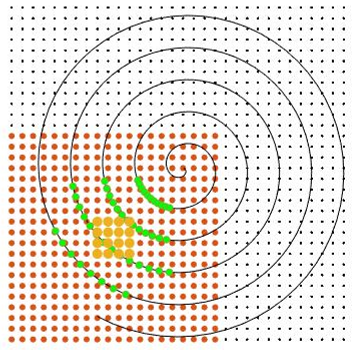
\includegraphics[width=6cm]{kspace_PTX_Patch}
	\caption{\textcolor{red}{WAG: I think you should make two subfigures here: one that illustrates a single target location, and one that illustrates a patch of target locations. Also you should annotate the different widths, in the figures, with arrows. Also add a legend for the dots} 
	Illustration of one instance within the palatalization of a 2D k-space domain design problem. The totally design problem is divided into patches of width 4 cycle/FOV, and the 16 yellow points are the target points in this instance. With inclusion width of 4 cycle/FOV, the 46 green excitation trajectory points within the 12 cycle/FOV wide green square (4 cycle/FOV extended outside of the patch) are considered in this instance. The excitation within the 20 cycle/FOV wide red patch is constrained to zero except the point where the delta function is.}
	\label{fig:Patch}
\end{figure}
An example of this concept is shown in Figure \ref{fig:Patch}. For simplicity of visualization, it is demonstrated in a 2D problem, but the concept is easily extended to 3D. The figure depicts the solution of the $\mathbf{W}$ matrix 16 columns at a time, whose corresponding delta functions live within a patch of width 4 cycle/FOV (yellow points in Figure \ref{fig:Patch}). In this instance where the inclusion width is also 4 cycle/FOV, we truncate the $B_1^+$ map Fourier transforms to zero outside a 4 by 4 cycle/FOV square centered at DC. As a result, we must consider all the excitation trajectory points within a 12 by 12 cycle/FOV square, which is 4 cycle/FOV extended outside of the patch width 4 square, since they may contribute energy to the target locations corresponding to the 16 $\mathbf{W}$ matrix columns. For a single instance of the 16-point target patch shown in Figure \ref{fig:Patch}, the 46 green points on the excitation trajectory may contribute significant energy and are considered in the weight design. Furthermore, we must constrain the total excitation to zero at all k-space locations within a 20 by 20 cycle/FOV red patch in Figure \ref{fig:Patch}. This is because any energy deposited at each considered excitation trajectory points will affect not only the target points in the yellow square, but also the whole 2$\times$4 wide patch around that trajectory point. And the 20 by 20 cycle/FOV red patch is the total of the points that can be affected by all the excitation trajectory points considered in this instance. Therefore, in the solution for this instance, $\mathbf{w}$ is a 46$N_c\times$16 matrix, $\mathbf{S}$ is a 400$N_c\times$46$N_c$ matrix, $\mathbf{S}^{H}\mathbf{S}$ is a 46$N_c\times$46$N_c$ matrix, and $\mathbf{s}_i^{H}$ is a 46$N_c\times$16 matrix. 
%Since $\mathbf{s}_i^{H}$ is no longer related to the $i$th row of $\mathbf{S}$ and $i$th column of $\mathbf{W}$ only, it will be denoted as $\mathbf{S_{targ}}$ in later discussions. 
In the next instance, another 16 columns centered around another 4 points by 4 points patch will be solved. It should be noted that in different instances, the number of neighboring excitation trajectory points (the 46 green points in the previous instance) can vary. We will denote this number of points by $N_n$. $N_n$ can be zero when a patch is at the corners where no excitation trajectory point is adjacent. 
%For patches near edges of the excitation k-space FOV, the solution neighborhood and area may wrap back in a circulant shift fashion, depending on the resolution of the final spatial grid on which the user will evaluate the pulse. In Figure \ref{fig:Patch}), denoted by the red area to the right of Figure \ref{fig:Patch}).

\par The patch width determines the total number of instances to be solved. The inclusion width determines the accuracy of $B_1^+$ information utilized in the design. Together, the patch width and the inclusion width determine how many excitation trajectory points are included in each instance, which further determines the size of $\mathbf{S}^{H}\mathbf{S}$ whose construction is most computationally burdensome within an instance. Therefore, increasing patch width reduces the number of $\mathbf{S}^{H}\mathbf{S}$ matrices to be constructed but increases the burden of constructing each of them. An optimal patch width should be decided case by case for different excitation trajectories. 

\subsection*{Efficient construction of $\mathbf{S}^{H}\mathbf{S}$ matrix}
\par Constructing $\mathbf{S}^{H}\mathbf{S}$ by finding $\mathbf{S}$ is computationally expensive. As described previously, the $((c-1)N_c+t)$-th column of the  $\mathbf{S}$ matrix, $\mathbf{S}_c(\vec{k}-\vec{k}_t)$, is the k-space sensitivity map of the $c$-th coil $\mathbf{S}_c(\vec{k})$ shifted to excitation k-space trajectory location $\vec{k}_t$. These shifts for each column of $\mathbf{S}$ are achieved by applying a linear phase modulation to the spatial domain $B_1^+$ map, followed by a fast Fourier transform (FFT). This process becomes computationally overwhelming when there are many RF samples, which is often the case. Furthermore, the matrix multiplication between $\mathbf{S}^{H}$ and $\mathbf{S}$ is also computationally intensive due to the large row dimension of $\mathbf{S}$ (400$Nt$ in the above example in Figure \ref{fig:Patch}).  


\par Inspired by a rapid GRAPPA calibration method for arbitrary 2D/3D non-Cartesian trajectories proposed in Ref \cite{luo2019grappa}, we have developed a fast and memory-efficient algorithm to solve this problem. A key innovation of Ref \cite{luo2019grappa} is that the algorithm constructs the Hermitian $\mathbf{S}^{H}\mathbf{S}$ matrix directly by finding each of the matrix's lower triangle elements through interpolation, instead of building the $\mathbf{S}$ matrix explicitly followed by matrix multiplication. Conceptually, each element in the Hermitian matrix $\mathbf{S}^{H}\mathbf{S}$ is the vector sum of two shifted k-space sensitivity maps, which is also one single point of their convolution. With the multiplication property of Fourier transform, this convolution in k-space can be calculated from the Fourier transform of the dot product of the two spatial domain $B_1^+$ maps. For a more detailed derivation, please refer to Ref \cite{luo2019grappa}.
In practice, $\mathbf{S}^{H}\mathbf{S}$ is constructed in the following way. We first represent the $\mathbf{S}^{H}\mathbf{S}$ matrix with block matrices. Each block matrix $\mathbf{S}_i^{H}\mathbf{S}_j$ is of size $N_n$ by $N_n$, and $\mathbf{S}_i$ and $\mathbf{S}_j$ are the columns of $\mathbf{S}$ related to the k-space sensitivity maps of the $i$-th and $j$-th coils respectively.

\begin{equation}
\mathbf{S}^{H}\mathbf{S} = 
\begin{pmatrix}
\mathbf{S}_1^{H}\mathbf{S}_1 & \cdots & \mathbf{S}_1^{H}\mathbf{S}_{N_c} \\
\vdots  &  \ddots & \vdots  \\
\mathbf{S}_{N_c}^{H}\mathbf{S}_1 & \cdots & \mathbf{S}_{N_c}^{H}\mathbf{S}_{N_c} 
\end{pmatrix}
\end{equation}

Since $\mathbf{S}^{H}\mathbf{S}$ is Hermitian, we only need to find the values within the lower triangle of the matrix, which are the lower triangle blocks $\mathbf{S}_i^{H}\mathbf{S}_j$ with $i>j$. For a given lower triangle block $\mathbf{S}_i^{H}\mathbf{S}_j$  ($i>j$), all of its elements are interpolated from the densely sampled Fourier transform of the dot product of the spatial domain $B_1^+$ maps of the $i$-th and $j$-th coils. The $(m,n)$-th element is the value interpolated at $(\vec{k}_m-\vec{k}_n)$ away from DC. Therefore, to solve all the columns of $\mathbf{W}$, the total number of FFT operations needed in this efficient method is only $N_c(N_c+1)/2$, instead of ${N_t}{N_c}$, and the storage size is also much smaller. In addition to the efficiency related to FFT, this algorithm saves a large matrix multiplication between $\mathbf{S}^{H}$ and $\mathbf{S}$ for the solving of every single column of $\mathbf{W}$. 
Although an alternative strategy of determining each column of $\mathbf{S}$ explicitly by interpolating the $N_s$ sample points from unshifted $B_1^+$ Fourier transforms can also reduce the number of FFT operations, it still has the problem of large multiplications between $\mathbf{S}^{H}$ and $\mathbf{S}$ matrices. Furthermore, to calculate each element of $\mathbf{S}^{H}\mathbf{S}$, there are $2N_s$ number of interpolations involved with this sub-optimal strategy. While with the efficient algorithm there is only one interpolation from the densely sampled Fourier Transform of the dot product of two spatial domain $B_1^+$ maps needed. The extra interpolations involved in the sub-optimal strategy would introduce a larger error to $\mathbf{S}^{H}\mathbf{S}$.  

\subsection*{ Off-Resonance correction}
\par As shown in Equation \ref{eq:SpatialDomainEquation} when we introduced spatial domain design in Chapter \ref{chap:SpatialDesign}, the equation connecting a pTx pulse to its excitation pattern has an off-resonance dependent term 
$e^{\imath \gamma \Delta B_0(\mathbf{x})(t-T)}$. In order to model this off-resonance dependent term in our k-space domain design, we adapted a fast implementation of the off-resonance compensation with time segmentation approximation and weighted least-squares interpolators \cite{fessler2005toeplitz}. 
By segmenting the RF pulse into multiple segments, this method disentangles the space-and-time dependent phase accrual induced by main field inhomogeneity into either space- or time- dependent terms, and therefore a same system matrix can be applied within each segment. Mathematically, it is
\begin{equation*}
e^{\imath \Delta\omega_j (t_i-T) }=\sum_{l=1}^{L} b_{l}(t_i) e^{\imath \theta_{l}(\Delta\omega_j)}
\end{equation*}
where $i=1\dots Nt$ indexes the RF samples, $j=1\dots Ns$ indexes the spatial locations, and $l$ indexes the time segments. The left term is the problematic space-and-time dependent term, with $\Delta\omega_j$ representing the off-resonance at the location-$j$ obtained from a field map and $T$ being the pulse duration. $b_{il}=b_{l}(t_i)$ are the time-dependent-only weights called temporal interpolators applied upon RF samples. $c_{lj}=e^{\imath \theta_{l}(\Delta\omega_j)}$ are the space-dependent-only phase accrual called spatial interpolators, applied upon the excitation pattern of each weighted RF segment. 
Therefore, the off-resonance correcting RF can be obtained by 
\begin{equation*}
\mathbf{b}=\sum_{l=1}^{L}diag\{\mathbf{b}_l\}\mathbf{W}\mathcal{F}(diag\{\mathbf{c}_l\}\mathbf{d})
\end{equation*}
where $\mathbf{b}_l$ and $\mathbf{c}_l$ are the vectorized interpoloators for the $l$-th segment. 



%!TEX root = kPtx_paper.tex
\section*{Methods}
\subsection*{Design and Simulation Setup}
Simulations were performed to validate and characterize the proposed k-space domain parallel transmit pulse design method,
with comparisons to the spatial-domain method of Ref. \cite{Grissom:2006:MRM}.
RF pulses were designed for a simulated 24-channel loop transmit array (Figure \ref{fig:Coil}) that is being built for a 7 Tesla scanner optimized
for imaging the human cortex.  
24-channel complex-valued $B_1^+$ maps used in the pulse designs were simulated in a male human head model using 
Ansys High Frequency Structure Simulator (Canonsburg, PA, USA) with 1.5 mm isotropic resolution. 
Figure \ref{fig:Target}a shows the target pattern for all pulse designs which comprised an ellipse centered on the ventricles with AP/HF/LR semi-axes of 4.8/3.2/3.2 cm,
\textcolor{blue}{with zero phase.}\revbox{R1.X} 
The pattern was smoothed by a Fermi filter that was applied in the frequency domain to match the target pattern's effective resolution to the excitation k-space trajectory's 5 mm resolution.
This choice of target pattern was motivated by imaging applications for the 7 Tesla scanner 
in which midbrain signals will be saturated for high-resolution, highly-accelerated imaging of the cortex. 
Pulses were designed to excite the entire ellipse and achieve zero excitation in voxels in the cerebrum but outside the ellipse. 
The smoothed target pattern and the $B_1^+$ maps were downsampled from their original 128$\times$128$\times$96 grids (1.5 mm isotropic resolution) to 
64$\times$64$\times$48 grids (3 mm isotropic resolution),
and RF designs were performed with the 64$\times$64$\times$48 grid size. 




\par A SPINS excitation k-space trajectory \cite{malik2012tailored} (Figure \ref{fig:Target}b) with 5 mm max resolution was used for the designs. 
The SPINS trajectory comprised three segments with radii ranging between 1-0.625, 0.625-0.375, and 0.375-0 cycles/cm, respectively.
The number of polar and azimuthal rotations were 15.5/2.125, 20.66/2.833, 15.5/2.125 for each segment, respectively.
The SPINS trajectories were first designed analytically and the final gradient waveforms and excitation k-space trajectories were designed from them 
using the minimum-time gradient waveform design method \cite{lustig2008fast}, 
for a 15 {\textmu}s dwell time and subject to the scanner's gradient amplitude and slew rate constraints of 200 mT/m and 700 T/m/s, respectively (Figure \ref{fig:Target}c). 
The durations of the three segments after minimum-time gradient design were 4.174, 4.326, and 1.5 ms, respectively.
With the exception of the simulations across undersampling factors, 
all pulse designs used this 10 ms trajectory.
With this trajectory and the 64$\times$64$\times$48 design grid size, 
the dimensions of the $\bm{W}$ matrix were 16,632 RF pulse samples, 
by 196,608 target k-space locations. 



\par All pulse designs and Bloch equation simulations were performed in MATLAB (Mathworks, Natick, MA, USA).
For spatial domain designs, 
RF pulses were solved using an iterative least-squares conjugate-gradient descent method \cite{Grissom:2006:MRM} with 35 iterations,
which was accelerated by non-uniform fast Fourier transforms \cite{Fessler:2003fk}. 
Except for the off-resonance-compensated designs described below, 
all spatial domain designs were parallelized using 16 threads that simultaneously computed the forward and backward 
non-uniform fast Fourier transforms across transmit coils. 
The proposed k-space domain algorithm was implemented based on code for the non-Cartesian GRAPPA method of Ref. \cite{luo2019grappa},
as a function that takes as input the $B_1^+$ maps, 
a normalized excitation k-space trajectory, \textcolor{blue}{and optional MATLAB structures of algorithm parameters such as the Tikhonov regularization parameter
and inclusion and patch widths, and off-resonance parameters such as the off-resonance field map, the time vector and the number of time segments.}\revbox{R1.X} 
Within that function the Fourier transforms of the $B_1^+$ products are calculated,
and a C-based \textcolor{blue}{MATLAB Executable (MEX)}\revbox{R1.X} function is invoked to solve for the non-zero elements of each column of $\bm{W}$,
with linear interpolation of the Fourier transforms of the $B_1^+$ map products to obtain the entries of the $\bm{S}^H\bm{S}$ matrices. 
Those elements are then inserted into a sparse $\bm{W}$ matrix, which is the single output of the main function. 
Parallelization was implemented across patches within the C-based MEX function using the \textcolor{blue}{Open Multi-Processing (OpenMP)}\revbox{R1.X} library. 
The final pulses are calculated by multiplying the sparse $\bm{W}$ matrix into the Fourier transform of the target pattern. 
This code, the $B_1^+$ maps, and a demo script are available at https://github.com/wgrissom/kpTx. 
All pulse designs were performed on a server (Colfax International, Santa Clara, CA, USA) 
with 512 GB RAM and two 24-core 2.1 GHz Intel Xeon CPUs which provide up to 94 threads (Intel Corporation, Santa Clara, CA, USA). 
Designs were performed five times for each case, and the mean computation time was recorded.
For the k-space domain designs, the design time comprised the time to compute the sparse $\bm{W}$ matrix, 
and the time to multiply it into the target pattern to obtain the pulses.
The resulting pulses were Bloch equation-simulated and compared to the target pattern on the finer 128$\times$128$\times$96 grid to capture Gibbs ringing. 
When calculating excitation errors, the magnitude root-mean-square error (RMSE) was calculated in voxels within the cerebrum,
except for an $\approx$5 mm-thick transition band around the edge of the elliptical target region.

\subsection*{k-Space Algorithm Parameters}
To evaluate how accuracy and compute time depend on k-space-domain design parameters and parallelization,
pulse designs were done across numbers of threads (i.e., how many patches were solved simultaneously; 1 to 32), 
patch widths (1 to 16 cycles/FOV), and inclusion widths (2 to 8 cycles/FOV). 
The number of threads were varied while holding the patch width and inclusion width both at 4 cycles/FOV.
The patch width was varied while holding the number of threads at 16, and the inclusion width at 4 cycles/FOV,
and the inclusion width was varied (2, 4, 6, and 8 cycles/FOV) while holding the number of threads at 16, and the patch width at 4 and 8 cycles/FOV. 
The sizes of the $\bm{W}$ matrices were also recorded, holding patch width constant at 4 cycles/FOV and varying the inclusion width. 

\subsection*{L-Curves}
To compare the tradeoff between excitation error (measured by root-mean-square error)
and integrated RF root-mean-square (RMS) amplitude for spatial and k-space domain designs,
pulse designs were repeated while varying Tikhonov regularization parameters ($\lambda$ in Equation \ref{eq:Solution}) 
over five orders of magnitude. 
The k-space domain designs were repeated four times to investigate the two main sources of error:
finite patch and inclusion widths, 
and $B_1^+$ map product interpolation when building the $\bm{S}^H\bm{S}$ matrices. 
Specifically, for each $\lambda$ a design was performed using patch and inclusion widths of four (`Patch/Inclusion Widths = 4')
with interpolated $B_1^+$ map products (`Interpolated Matrices'),
patch and inclusion widths covering the entire design grid (`Patch/Inclusion Widths = $\infty$') with interpolated $B_1^+$ map products,
patch and inclusion widths of four without $B_1^+$ map product interpolation (`Exact Matrices'; 
$B_1^+$ maps were phase-modulated to each trajectory location before Fourier transform),
and patch and inclusion widths covering the entire design grid without $B_1^+$ map product interpolation. 
Note that the last case is equivalent to the original k-space domain method of Ref. \cite{Katscher:2003:Magn-Reson-Med:12509830}.
For each design, flip angle RMSE (calculated using the spatial domain non-uniform fast Fourier transform) and root-mean-square RF amplitude were
recorded.

\subsection*{Gibbs Ringing}
Gibbs ringing commonly arises in spatial domain parallel pulse designs when the resolution of the 
design grid is similar to that of the excitation k-space trajectory. 
The proposed k-space-domain method is implemented without wraparound or circulant end conditions in excitation k-space, 
so Gibbs ringing should be suppressed even when using a design grid that is only slightly wider than the trajectory. 
To demonstrate this, 
the target pattern and $B_1^+$ maps were further down-sampled to 32$\times$32$\times$24 (6 mm isotropic-resolution),
and the outermost leaves of the SPINS trajectory which had duration 2.1 ms were excluded so that the maximum excitation 
resolution matched the 6 mm target pattern and $B_1^+$ map resolution. 
Using this shorter 7.9 ms trajectory, 
pulses were designed by the spatial domain method using both 32$\times$32$\times$24 and 64$\times$64$\times$48 grid sizes,
and by the k-space-domain method for 32$\times$32$\times$24 grid size.
The Tikhonov regularization parameters for the 32$\times$32$\times$24 designs were set so that the RMS RF amplitudes produced 
by the k-space domain and spatial domain designs matched.
The designed pulses were then evaluated against the target pattern using the 128$\times$128$\times$96 grid size,
to visualize the ringing.

\subsection*{Excitation k-Space Undersampling}
An important application of parallel transmission is the reduction of multidimensional pulse durations by excitation k-space undersampling.
To compare the spatial domain and k-space domain methods across undersampling factors,
the number of polar and azimuthal rotations were increased and reduced relative to the reference design described above, 
for reduction factors of 0.5, 2, 3, and 4. 

\subsection*{Off-Resonance}
To compare the off-resonance-compensated k-space domain designs with off-resonance-compensated spatial domain designs,
we incorporated a Gaussian ($\sigma = 3$ cm) field map centered above the frontal sinus, 
which was designed to mimic the characteristic susceptibility-induced $B_0$ inhomogeneity in this part of the human brain. 
The field maps were than scaled so that the maximum off-resonance reached +200 Hz and +400 Hz.
A time-segmented approximate off-resonance model was calculated using the method of Ref. \cite{fessler2005toeplitz} with $L = 4$ time segments,
and this model was used in both spatial domain and k-space domain designs. 
Both spatial domain and k-space domain designs used 32 parallel threads. 




%!TEX root = kPtx_paper.tex
\section*{Results}


Figure \ref{fig:ErrorMap} shows simulated excitation patterns and error maps for the reference spatial and k-space domain designs. 
Both designs were performed with 16 parallel threads and the 64$\times$64$\times$48 grid size (3 mm isotropic resolution), 
and the excitation patterns were evaluated against the target pattern on a 128$\times$128$\times$96 grid size (1.5 mm iso-resolution). 
The k-space domain design used patch and inclusion widths of 4.
The calculated root-mean-squared errors (RMSEs) were 2.42\% (spatial domain) and 2.68\% (k-space domain), 
respectively. 
For both design methods, most of the errors appeared at the edges of the transition band, 
and errors elsewhere were lower than 5\% of the target flip angle. 
This indicates uniform inner volume excitation while maintaining the outer volume intact. 
The parallelized k-space domain design required 2.9 seconds computation versus 31.8 seconds for the spatial domain method, a 91\% decrease.


\subsection*{k-Space Algorithm Parameters}
Figure \ref{fig:ComputationTime}a plots mean computation time versus number of parallel threads,
holding the patch and inclusion widths fixed at 4 cycles/FOV. 
The computation time decreased rapidly with increasing thread number up to 12 threads, 
and then plateaued, likely due to the overhead involved in initiating threads after that point.
Based on this result, the number of threads was held fixed at 16 for subsequent designs when off-resonance was not compensated.

\par Figure \ref{fig:ComputationTime}b plots mean computation time and RMSE with different patch widths. 
The computation time decreased up to a patch width of 4 cycles/FOV (corresponding to $4^3 = 64$ simultaneously solved columns of $\bm{W}$) 
and then increased sharply for larger patch widths. 
RMSE decreased slowly as the patch width increased since the number of excitation trajectory points included in the calculation of weights for each 
target point increases on average (and especially for target locations in the middle of each patch) as the patch width increases, 
even when the inclusion width stays fixed.
Based on this result, a patch width of 4 cycles/FOV was used for subsequent designs.

\par Figure \ref{fig:ComputationTime}c plots mean computation time and RMSE with different inclusion widths. 
The solid lines and dashed lines were obtained with patch widths of 4 and 8 cycles/FOV, respectively. 
Computation time increased and error decreased with increasing inclusion width,
since more excitation trajectory points were included in each target location's calculation for increasing inclusion width,
corresponding to an increased $\bm{S}^H\bm{S}$ matrix size. 
The RMSE was only slightly lower for a patch width of 8 versus 4 cycles/FOV, 
but the computation time was much higher for 8 cycles/FOV, across all inclusion widths. 
The knees in the curves occurred approximately at an inclusion width of 4 cycles/FOV,
so this value was used in subsequent designs. 

\par Table \ref{fig:wsize} lists the size of the final matrix $\bm{W}$ in gigabytes,
versus inclusion width.
As inclusion width increases, more excitation trajectory points are used in the solution of the weights for each target location,
until the entire trajectory is used for each location (inclusion width = $\infty$ in the table),
corresponding to a full solution. 
With the inclusion width of 4 cycles/FOV used here, 
the matrix size was 98\% smaller than that of a full solution.  





\subsection*{L-Curves}
Figure \ref{fig:LCurves} plots flip angle RMSE versus RF RMS amplitude for the spatial domain method
and different configurations of the k-space domain method.
The spatial domain method achieves the best overall tradeoff between error and RMS amplitude (dashed black curve),
which is matched by the k-space domain method when all target locations are solved simultaneously with
all excitation trajectory points included and exact $\bm{S}^H\bm{S}$ matrix construction (orange curve). 
When the inclusion and patch widths are limited to 4 cycles/FOV but the $\bm{S}^H\bm{S}$ 
matrices are still constructed exactly, there is an increase in error and RMS amplitude (solid blue curve). 
However, a larger penalty is incurred by interpolating the entries of the $\bm{S}^H\bm{S}$ matrices (dashed orange curve)
than by limiting the inclusion and patch widths.
Combining interpolation of the $\bm{S}^H\bm{S}$ matrix entries and patch and inclusion widths of 4 cycles/FOV yield 
the dashed blue curve, which has a higher error and RF amplitude than when interpolation or small patch and inclusion widths are
used alone.
Overall, these results and the results in Figure \ref{fig:ComputationTime} and Table \ref{fig:wsize}
show that the k-space domain method allows a tradeoff between computation time and memory usage versus
excitation error and RMS RF amplitude.
The dots on the spatial domain and k-space domain curves indicate the knees \textcolor{blue}{of}\revbox{R1.9} the curves corresponding to
the $\lambda$ values used for the designs in Figures \ref{fig:ErrorMap}, \ref{fig:ComputationTime}, \ref{fig:kspace_PTX_Acceleration}, and \ref{fig:kspace_PTX_B0}.
Note that the RMSE's in Figure \ref{fig:LCurves} are slightly lower for the spatial domain designs
and slightly higher for the k-space domain designs compared to other figures,
because the flip angle errors in Figure \ref{fig:LCurves} were calculated using 
spatial domain NUFFTs instead of Bloch equation simulations, 
to provide a more direct measure of the design error. 



\subsection*{Gibbs Ringing}
Figure \ref{fig:GibbsRing}a shows slices of the excitation error pattern produced by pulses designed by the spatial domain method
on a 32$\times$32$\times$24 grid, which were Bloch-simulated on the original 128$\times$128$\times$96 grid. 
There is significant Gibbs ringing in the pattern (indicated by the red arrows),
and the pulses incur a higher RMSE (4.64\%) than pulses designed using either the spatial domain method with a finer 64$\times$64$\times$48 grid
(2.66\%; Figure \ref{fig:GibbsRing}b) or the k-space domain method with a 32$\times$32$\times$24 grid (3.00\%; Figure \ref{fig:GibbsRing}c). 
Gibbs ringing is not apparent in either the 64$\times$64$\times$48 spatial domain error pattern or the 32$\times$32$\times$24 k-space domain error pattern. 
The RMS RF amplitudes of the low resolution designs were both 0.005. 
Note that the error of the 64$\times$64$\times$48 spatial domain design is slightly higher than designs presented in other figures
due to the lower-resolution excitation trajectory. 
From a spatial domain point of view, 
the Gibbs ringing in the low-resolution spatial domain design was caused by the design's inability to observe and limit the ringing in the low-resolution design grid. 
From a k-space domain point of view, the Gibbs ringing was due to implicit circulant end conditions at the edges of excitation k-space,
which led RF samples at one edge of k-space to wrap-around and affect target locations at the opposite edge of k-space. 
This effect is mitigated using a high-resolution spatial domain design grid, as illustrated in Figure \ref{fig:GibbsRing}b. 
However, even for a low-resolution k-space domain design there is no wrap-around effect in excitation k-space 
because the trajectory points that are incorporated in solution for each patch are explicitly specified to be those in the immediate vicinity of 
that patch, without circulant end conditions. 
%Particularly, for the instance problems whose patches are at the edges of the k-space FOV, the excitation trajectory points at the other ends of the k-space FOV will not be incorporated into the design.    

%Due to implicit circulant end conditions in k-space for the spatial domain design, t



\subsection*{Excitation k-Space Undersampling}
Figure \ref{fig:kspace_PTX_Acceleration} compares excitation error patterns produced by spatial domain-designed pulses (top row)
and k-space domain-designed pulses (middle row),
for different trajectory reduction factors which resulted in the SPINS trajectories plotted in the third row. 
For each design the k-space domain-designed pulses had higher error, 
but error increased smoothly with increasing reduction factor, 
as it did for the spatial domain designs. 
\textcolor{blue}{Figure \ref{fig:kspace_PTX_Acceleration} also reports mean computation time for each design.
The spatial domain times were fairly constant across reduction factors despite the decreasing number of time samples with increasing reduction factor.
This was because the size of the FFT operations in the NUFFTs 
depended not on the length of the trajectory but on the size of the target pattern which did not change with reduction factor,
and the FFT operations dominated the NUFFT computation times relative to the gridding operations. % for these three-dimensional problems,
Conversely, the k-space domain times did decrease with reduction factor since the number and sizes of the $\bm{S}^H\bm{S}$
matrices depend on the trajectory length.} \revbox{R2.1}



\subsection*{Off-Resonance}
Figure \ref{fig:kspace_PTX_B0}a shows the off-resonance maps containing a Gaussian distortion which was centered above the frontal sinus,
and scaled to peak amplitudes of 0, 200, and 400 Hz for the pulse designs and Bloch simulations. 
Figure \ref{fig:kspace_PTX_B0}b shows excitation error patterns and RMSEs for spatial domain designs with off-resonance compensation,
and k-space domain designs without and with off-resonance compensation. 
Without off-resonance compensation, 
the k-space domain-designed pulses produced large ($>$ 10\% of $M_0$) excitation errors both inside and outside the target ellipse. 
When the off-resonance map was incorporated in the spatial domain and k-space domain designs, 
the distortion was nearly fully corrected when it had a peak amplitude of 200 Hz. 
When the map was scaled to a peak of 400 Hz, some large errors remained, with the k-space domain-designed pulses achieving slightly lower RMSE. 
%It was also able to provide excitation pattern comparable to spatial domain design with 400 Hz maximum off-resonance. The k-space domain design has a weaker performance with higher off-resonance due to the fact that the time segmentation approximation in Ref \cite{fessler2005toeplitz} was meant to approximate forward models from RF to excitation patterns and does not serve as an accurate approximation to the backward model as we need in the k-space domain design.

%!TEX root = kPtx_paper.tex
\section*{Discussion}
\subsection*{Summary}
A small-tip-angle k-space domain parallel transmit pulse design algorithm was proposed
that divides up the calculation of a matrix relating a target excitation pattern to the pulses that produce it 
into a set of independent problems for patches of target excitation k-space locations,
each of which is influenced by a local neighborhood of points on the excitation k-space trajectory.
The division of the problem into patches of target locations creates an opportunity for fine parallelization,
while the limited neighborhood sizes lead to small problem sizes for each patch. 
Compared to the original k-space-based algorithm of Ref. \cite{Katscher:2003:Magn-Reson-Med:12509830},
the L-curve and matrix size results showed that 
the new algorithm produces much smaller matrix sizes that can be calculated more quickly,
with the tradeoff of increased excitation error or RF power. 
Results showed that the algorithm also enables compensation of off-resonance 
which has not previously been described in a k-space domain design. 
Compared to a spatial domain design,
the new algorithm is non-iterative and can be finely parallelized to achieve shorter design times, 
and results showed that it can use coarser target grid sizes while avoiding Gibbs ringing, 
again with the tradeoff of increased excitation error or RF power.
The performance of off-resonance-compensated spatial domain and k-space domain pulse designs was similar,
and the methods were similarly sensitive to excitation k-space undersampling. 
\textcolor{blue}{While all the pulse designs in this work used 3D SPINS trajectories,
the method can be applied in any number of dimensions and with any excitation k-space trajectory.
The MATLAB implementation described can be used for any two- or three-dimensional pulse design without modification.}\revbox{R1.2}

\subsection*{Applications and Extensions}
This work was initially motivated by the observation that spatial domain parallel pulse designs can be very slow
for 3D problems with large grid sizes, 
requiring both many iterations and considerable computation per iteration. 
It is anticipated that the proposed k-space domain algorithm will be most useful for these types of large $>$2D problems,
which include 3D spatial designs \cite{malik2012tailored,davids2016fast} 
and \textcolor{blue}{2D and 3D spatial-spectral designs \cite{stenger2000three,setsompop2009,Malik:2010aa,yang2010four}
where full matrix construction and inversion is infeasible due to the problem size, }\revbox{R1.7}
and an iterative design can require several minutes to solve. 
\textcolor{blue}{Furthermore, unlike an iterative spatial domain design the proposed algorithm does not need to be repeated if the target pattern changes.
This means it could have a considerable computational speed advantage for Gerchberg-Saxton magnitude least-squares pulse designs \cite{setsompop2008magnitude,malik:mrm:2015}
which alternate between designing pulses and updating a complex-valued target pattern.
Such a design method would allow the user to specify only the magnitude of the target pattern, 
rather than magnitude and phase as was required in this work.}\revbox{R1.1}
The method could also be used to initialize spatial-domain designs to reduce the number of iterations required to reach a target cost. 
Finally, while simple Tikhonov RF power regularization was used in the designs presented here,
more sophisticated regularization could be incorporated to, 
e.g., control peak RF power via adaptive regularization \cite{Yip:2005:Magn-Reson-Med:16155881},
or to enforce array compression by projecting the weights into the null space of a compression matrix \cite{cao2016array},
\textcolor{blue}{among other applications \cite{padormo:2016,deniz:2019}.} \revbox{R1.8}
In such designs, it would be beneficial to pre-compute and store the lower triangular elements of the $\bm{S}^H\bm{S}$ matrices
so they need not be re-computed as the regularization changes over iterations.  
\textcolor{blue}{Peak power could also be controlled in k-space domain designs using parallel transmission 
VERSE \cite{Lee:2011:MRM} or the iterative re-VERSEit technique \cite{lee2009tod}.} \revbox{R1.8, R2.2}
\textcolor{blue}{It is not yet clear whether or how hard constraints on SAR and 
peak- and integrated-power could be directly incorporated in the k-space method, as in Refs \cite{brunner2010optimal} and \cite{hoyos:tmi:2014}. }\revbox{R1.8, R2.2}
\textcolor{blue}{It may also be possible to use the k-space domain method to rapidly design large-tip-angle pulses via the direct linear class of large-tip-angle pulses method \cite{Xu:2008aa} or the additive angle method \cite{grissom:mrm:2008}; 
the latter alternates between small-tip-angle designs that could be solved by the k-space method, 
and Bloch simulations to update the target pattern.} \revbox{R2.3}


\section*{Conclusion}
The proposed k-space domain algorithm accelerates and finely parallelizes parallel transmission pulse design,
with a modest tradeoff of excitation error and RMS RF amplitude.


\section*{Acknowledgments}
The authors would like to thank Tianrui Luo at University of Michigan for helpful discussions regarding Ref \cite{luo2019grappa}.



\pagebreak

\bibliographystyle{cse}
%\bibliography{kPtx_paper}

\begin{thebibliography}{10}
\providecommand{\url}[1]{\texttt{#1}}
\providecommand{\urlprefix}{URL }

\bibitem{Katscher:2003:Magn-Reson-Med:12509830}
Katscher U, B{\"o}rnert P, Leussler C, van~den Brink JS.
\newblock Transmit {SENSE}.
\newblock Magn Reson Med 2003;\hspace{0pt}49:144--150.

\bibitem{zhu2004parallel}
Zhu Y.
\newblock Parallel excitation with an array of transmit coils.
\newblock Magn Reson Med 2004;\hspace{0pt}51:775--784.

\bibitem{malik:mrm:2015}
Malik SJ, Hajnal JV.
\newblock Phase relaxed localized excitation pulses for inner volume fast spin
  echo imaging.
\newblock Magn Reson Med 2016;\hspace{0pt}76:848--861.

\bibitem{mooiweer:2016}
Mooiweer R, Sbrizzi A, Raaijmakers AJE, Van~den Berg CAT, Luijten PR, Hoogduin
  H.
\newblock Combining a reduced field of excitation with {SENSE}-based parallel
  imaging for maximum imaging efficiency.
\newblock Magn Reson Med 2016;\hspace{0pt}78:88--96.

\bibitem{Zhang:2007:Magn-Reson-Med:16526012}
Zhang Z, Yip CY, Grissom W, Noll DC, Boada FE, Stenger VA.
\newblock Reduction of transmitter {B1} inhomogeneity with transmit {SENSE}
  slice-select pulses.
\newblock Magn Reson Med 2007;\hspace{0pt}57:842--847.

\bibitem{cloos:kpstd:2012}
Cloos MA, Boulant N, Luong M, Ferrand G, Giacomini E, Le~Bihan D, Amadon A.
\newblock {$k_T$}-{Points}: {Short} three-dimensional tailored {RF} pulses for
  flip-angle homogenization over an extended volume.
\newblock Magn Reson Med 2011;\hspace{0pt}67:72--80.

\bibitem{deng:2009}
Deng W, Yang C, Alagappan V, Wald LL, Boada FE, Stenger VA.
\newblock Simultaneous z-shim method for reducing susceptibility artifacts with
  multiple transmitters.
\newblock Magn Reson Med 2009;\hspace{0pt}61:255--259.

\bibitem{Grissom:2006:MRM}
Grissom WA, Yip CY, Zhang Z, Stenger VA, Fessler JA, Noll DC.
\newblock Spatial domain method for the design of {RF} pulses in multicoil
  parallel excitation.
\newblock Magn Reson Med 2006;\hspace{0pt}56:620--9.

\bibitem{malik2012tailored}
Malik SJ, Keihaninejad S, Hammers A, Hajnal JV.
\newblock Tailored excitation in {3D} with spiral nonselective {(SPINS) RF}
  pulses.
\newblock Magn Reson Med 2012;\hspace{0pt}67:1303--1315.

\bibitem{davids2016fast}
Davids M, Schad LR, Wald LL, Guerin B.
\newblock Fast three-dimensional inner volume excitations using parallel
  transmission and optimized k-space trajectories.
\newblock Magn Reson Med 2016;\hspace{0pt}76:1170--1182.

\bibitem{orzada:2019}
Orzada S, Solbach K, Gratz M, Brunheim S, Fiedler TM, Johst S, Bitz AK,
  Shooshtary S, Abuelhaija A, Voelker MN, Rietsch SHG, Kraff O, Maderwald S,
  Fl\"oser M, Oehmigen M, Quick HH, Ladd ME.
\newblock A 32-channel parallel transmit system add-on for 7t mri.
\newblock PLOS ONE 2019;\hspace{0pt}14:1--20.

\bibitem{deng:2011}
Deng W, Yang C, Stenger VA.
\newblock Accelerated multidimensional radiofrequency pulse design for parallel
  transmission using concurrent computation on multiple graphics processing
  units.
\newblock Magn Reson Med 2011;\hspace{0pt}65:363--369.

\bibitem{setsompop2008magnitude}
Setsompop K, Wald L, Alagappan V, Gagoski B, Adalsteinsson E.
\newblock Magnitude least squares optimization for parallel radio frequency
  excitation design demonstrated at 7 {Tesla} with eight channels.
\newblock Magn Reson Med 2008;\hspace{0pt}59:908--915.

\bibitem{brunner2010optimal}
Brunner DO, Pruessmann KP.
\newblock Optimal design of multiple-channel {RF} pulses under strict power and
  {SAR} constraints.
\newblock Magn Reson Med 2010;\hspace{0pt}63:1280--1291.

\bibitem{hoyos:tmi:2014}
Hoyos-Idrobo A, Weiss P, Massire A, Amadon A, Boulant N.
\newblock On variant strategies to solve the magnitude least squares
  optimization problem in parallel transmission pulse design under strict {SAR}
  and power constraints.
\newblock IEEE Trans Med Imag 2014;\hspace{0pt}33:739--748.

\bibitem{fessler2005toeplitz}
Fessler JA, Lee S, Olafsson VT, Shi HR, Noll DC.
\newblock Toeplitz-based iterative image reconstruction for {MRI} with
  correction for magnetic field inhomogeneity.
\newblock IEEE Trans Sig Proc 2005;\hspace{0pt}53:3393--3402.

\bibitem{grissom:ismrm18}
Grissom WA.
\newblock {k-Space} domain parallel transmit pulse design.
\newblock In Proceedings 26th Scientific Meeting, International Society for
  Magnetic Resonance in Medicine, Paris. 2018;\hspace{0pt} p. 3396.

\bibitem{luo2019grappa}
Luo T, Noll DC, Fessler JA, Nielsen JF.
\newblock A {GRAPPA} algorithm for arbitrary {2D/3D} non-{Cartesian} sampling
  trajectories with rapid calibration.
\newblock Magn Reson Med 2019;\hspace{0pt}82:1101--1112.

\bibitem{lustig2008fast}
Lustig M, Kim SJ, Pauly JM.
\newblock A fast method for designing time-optimal gradient waveforms for
  arbitrary k-space trajectories.
\newblock {IEEE} Trans Med Imag 2008;\hspace{0pt}27:866--873.

\bibitem{Fessler:2003fk}
Fessler JA, Sutton BP.
\newblock Nonuniform fast {Fourier} transforms using min-max interpolation.
\newblock IEEE Trans Sig Proc 2003;\hspace{0pt}51:560--574.

\bibitem{stenger2000three}
Stenger VA, Boada FE, Noll DC.
\newblock Three-dimensional tailored {RF} pulses for the reduction of
  susceptibility artifacts in {$T_2^*$}-weighted functional {MRI}.
\newblock Magn Reson Med 2000;\hspace{0pt}44:525--531.

\bibitem{yang2010four}
Yang C, Deng W, Alagappan V, Wald LL, Stenger VA.
\newblock Four-dimensional spectral-spatial {RF} pulses for simultaneous
  correction of {B1+} inhomogeneity and susceptibility artifacts in
  {T2*}-weighted {MRI}.
\newblock Magn Reson Med 2010;\hspace{0pt}64:1--8.

\bibitem{Yip:2005:Magn-Reson-Med:16155881}
Yip CY, Fessler JA, Noll DC.
\newblock Iterative {RF} pulse design for multidimensional, small-tip-angle
  selective excitation.
\newblock Magn Reson Med 2005;\hspace{0pt}54:908--917.

\bibitem{cao2016array}
Cao Z, Yan X, Grissom WA.
\newblock Array-compressed parallel transmit pulse design.
\newblock Magn Reson Med 2016;\hspace{0pt}76:1158--1169.

\bibitem{Lee:2011:MRM}
D.~Lee, W.~A. Grissom, M.~Lustig, A.~B. Kerr, P.~P. Stang, and J.~M. Pauly.
\newblock {VERSE}-guided numerical {RF} pulse design: A fast method for peak
  {RF} power control.
\newblock Magn Reson Med 2012; 67:353--362.

\bibitem{lee2009tod}
D.~Lee, M.~Lustig, W.~A. Grissom, and J.~M. Pauly.
\newblock Time-optimal design for multidimensional and parallel transmit
  variable-rate selective excitation.
\newblock Magn Reson Med 2009, 61(6):1471--1479.

\bibitem{Xu:2008aa}
D.~Xu, K.~F. King, Y.~Zhu, G.~C. McKinnon, and Z.-P. Liang.
\newblock Designing multichannel, multidimensional, arbitrary flip angle {RF}
  pulses using an optimal control approach.
\newblock Magn Reson Med 2008, 59(3):547--560.

\bibitem{grissom:mrm:2008}
W.~A. Grissom, C.~Y. Yip, S.~M. Wright, J.~A. Fessler, and D.~C. Noll.
\newblock Additive angle method for fast large-tip-angle {RF} pulse design in
  parallel excitation.
\newblock Magn Reson Med 2008, 59(4):779--87.





\end{thebibliography}


\pagebreak
%(Please see main document for caption with intended math typesetting)

\begin{figure}
	\centering
	%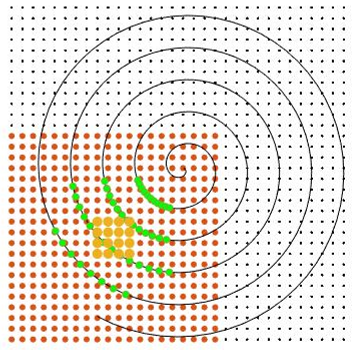
\includegraphics[width=\textwidth]{kspace_PTX_Patch}
	\caption{(a) A target point $\vec{k}_j$ and the nearby trajectory points that are included when calculating 
	RF pulse weight contributions from this point.
	Inclusion width is defined as the distance from each target location $\vec{k}_j$ within which 
	which all trajectory points are considered when solving for the $j$-th column of the design ($\bm{W}$) matrix.
	(b) Calculation of the $\bm{W}$ matrix can be performed column-by-column for each target location $\vec{k}_j$,
	or patches of target points can be solved for jointly. 
	Here the 16 columns of $\bm{W}$ for a 4 $\times$ 4 patch of target points are solved together,
	and an inclusion width of 4 cycles/FOV dictates that all trajectory points within a 12 $\times$ 12 region
	centered on the patch are considered in the calculation.}
	\label{fig:Patch}
\end{figure}

\begin{figure}
	\centering
	%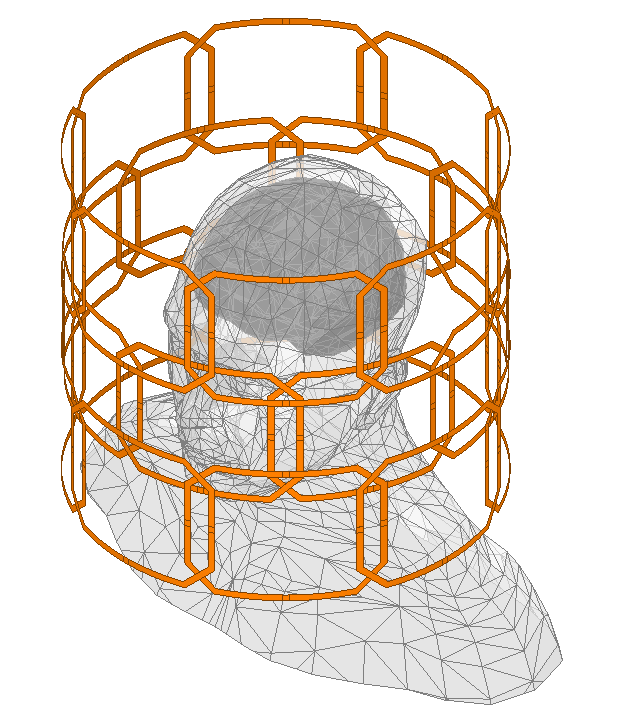
\includegraphics[width=6cm]{kspace_PTX_Coil}
	\caption{The 24-channel loop Tx array that was simulated in a human head model to obtain $B_1^+$ maps. 
	The array has diameter 32 cm and height 28 cm. The 16 cm $\times$ 11 cm rectangular loops are arranged in 3 rows of 8.}
	\label{fig:Coil}
\end{figure}

\begin{figure}
	\centering
	%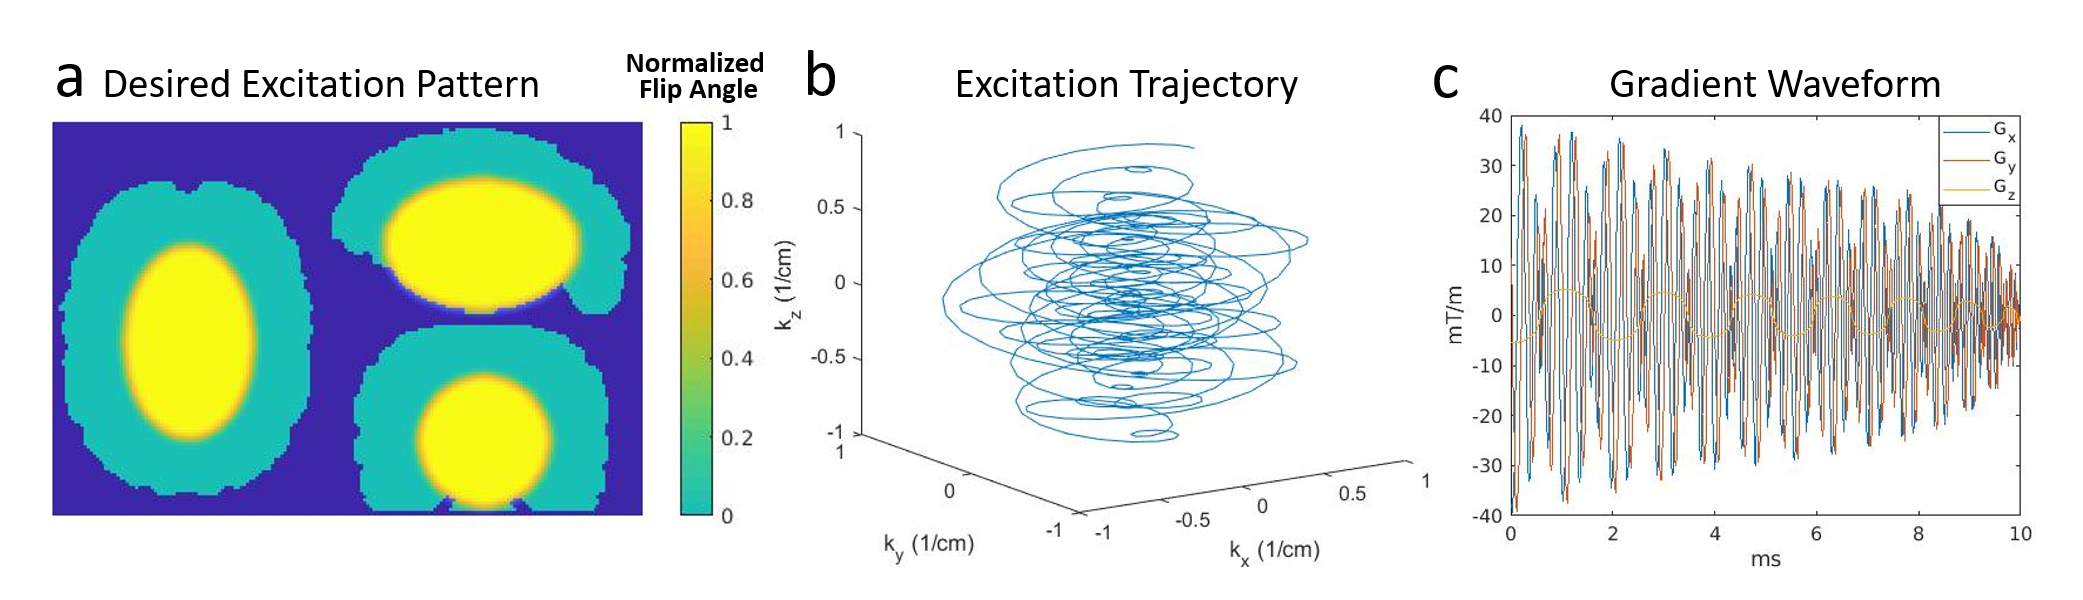
\includegraphics[width=\textwidth]{kSpace_PTX_Pattern_Trajectory}
	\caption{(a) Middle axial, sagittal, and coronal slices of the target excitation pattern used for all pulse designs. 
	(b) The SPINS trajectory used in the designs. 
	(c) 10 ms minimum-time gradient waveforms that produce the SPINS trajectory.}
	\label{fig:Target}
\end{figure}

\begin{figure}
	\centering
	%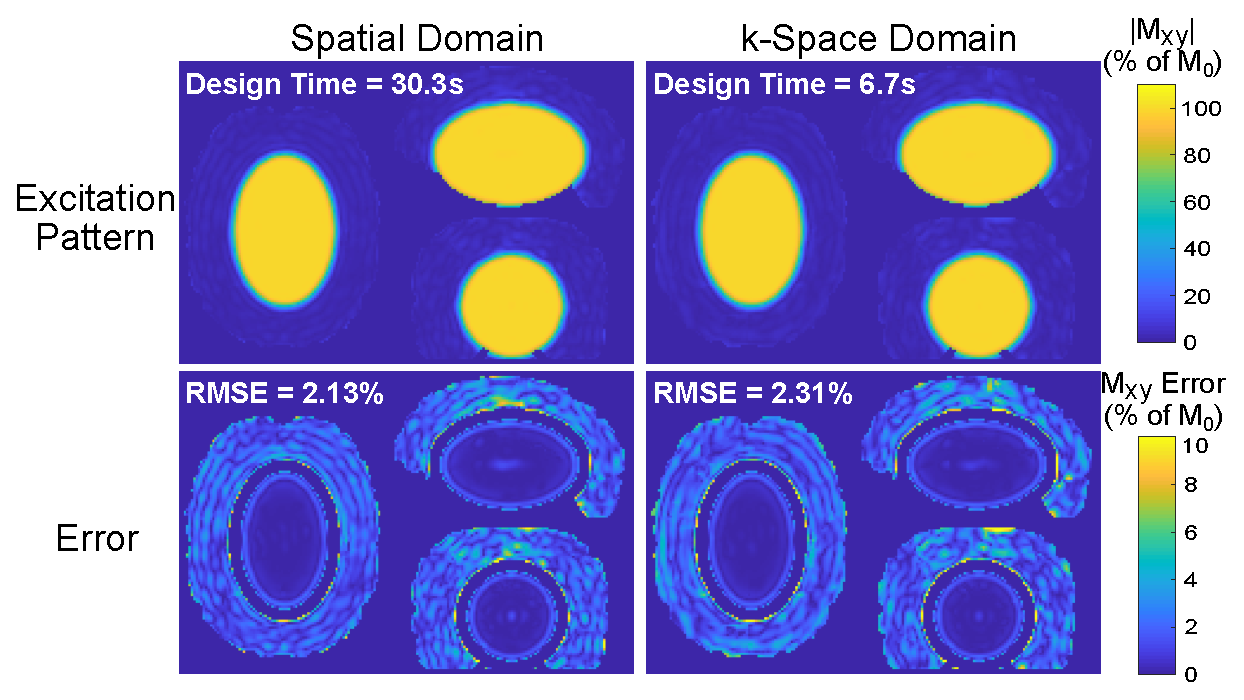
\includegraphics[width=\textwidth]{ErrorMap}
	\caption{ %\textcolor{red}{WAG: I think this is the figure that your example in Github should replicate.}
	Normalized excitation patterns (top row) and error maps (bottom row) in central axial, sagittal and coronal slices 
	for k-space domain (left) and spatial domain designs (right).}
	\label{fig:ErrorMap}
\end{figure}

\begin{figure}
	\centering
	%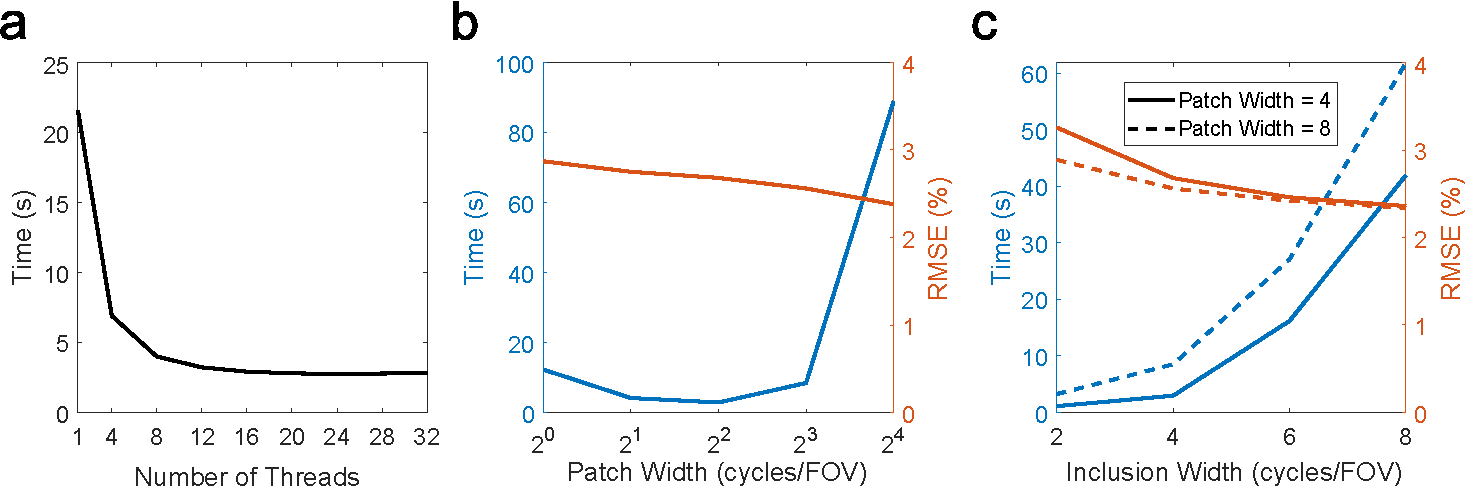
\includegraphics[width=\textwidth]{ComputationTime}
	\caption{(a) k-Space computation time versus number of parallel threads, for patch and inclusion widths of 4 cycles/FOV. 
	(b) Computation time (blue axis) and RMSE (red axis) versus patch width, for an inclusion width of 4 cycles/FOV and 16 threads. 
	(c) Computation time (blue axis) and RMSE (red axis) versus inclusion width, for patch widths of 4 and 8 cycles/FOV, and 16 threads.}
	\label{fig:ComputationTime}
\end{figure}

\begin{figure}
\centering
%\begin{tabular}{c | c}
%Inclusion Width & $\bm{W}$ Matrix Size (GB) \\
%\hline
%$\infty$ & 24.4 \\
%8 & 2.73 \\
%6 & 1.37 \\
%4 & 0.53 \\
%2 & 0.14
%\end{tabular}
\caption{$\bm{W}$ matrix sizes in gigabytes (GB) versus inclusion width in cycles/FOV. 
An inclusion width of $\infty$ corresponds to a full matrix solution.}
\label{fig:wsize}
\end{figure}

\begin{figure}
	\centering
	%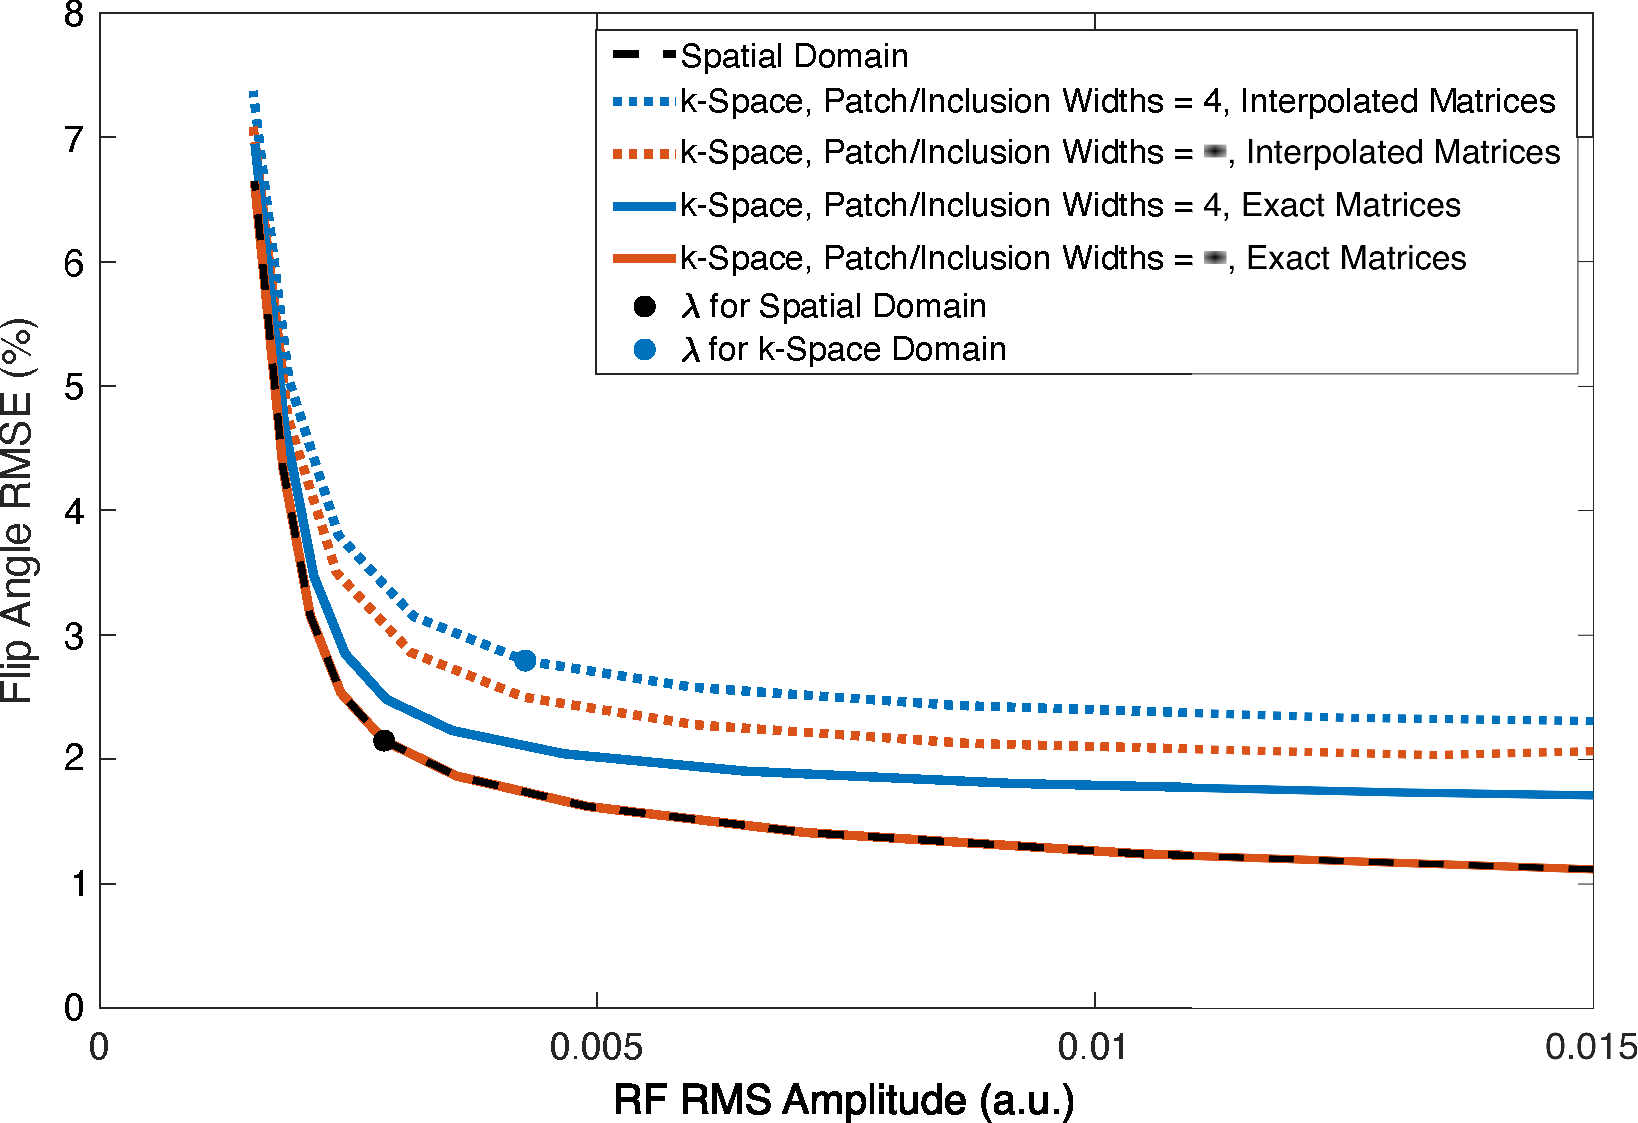
\includegraphics[width=\textwidth]{L_curve}
	\caption{L-curves for spatial domain and k-space domain pulse designs, 
	repeated across five orders of magnitude of the methods' Tikhonov regularization parameters.
	The k-space domain designs were repeated using patch and inclusion widths of four versus solving for the entire domain at once (`Patch / Inclusion Widths = 4' versus `Patch / Inclusion Widths = $\infty$'),
	and using $B_1^+$ map product interpolation versus phase modulation to each trajectory location (`Interpolated Matrices' versus
	`Exact Matrices').}
	\label{fig:LCurves}
\end{figure}


\begin{figure}
	\centering
	%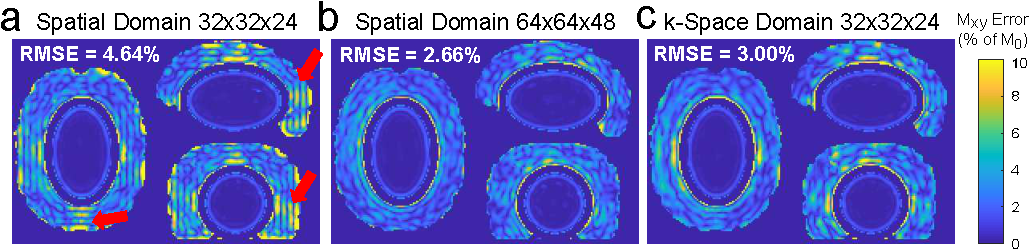
\includegraphics[width=\textwidth]{GibbsRinging}
	\caption{Normalized error maps and RMSEs for 
	(a) pulses designed using a trajectory that reaches 6 mm isotropic resolution
	and the spatial domain algorithm with a 32$\times$32$\times$24 grid, 
	(b) pulses designed using the same trajectory and the spatial domain algorithm with a 64$\times$64$\times$48 grid,  
	and (c) pulses designed using the same trajectory and the k-space domain algorithm with a 32$\times$32$\times$24 design grid. 
	Red arrows indicate Gibbs ringing in the 32$\times$32$\times$24 spatial domain design.}
	\label{fig:GibbsRing}
\end{figure}


\begin{figure}
	\centering
	%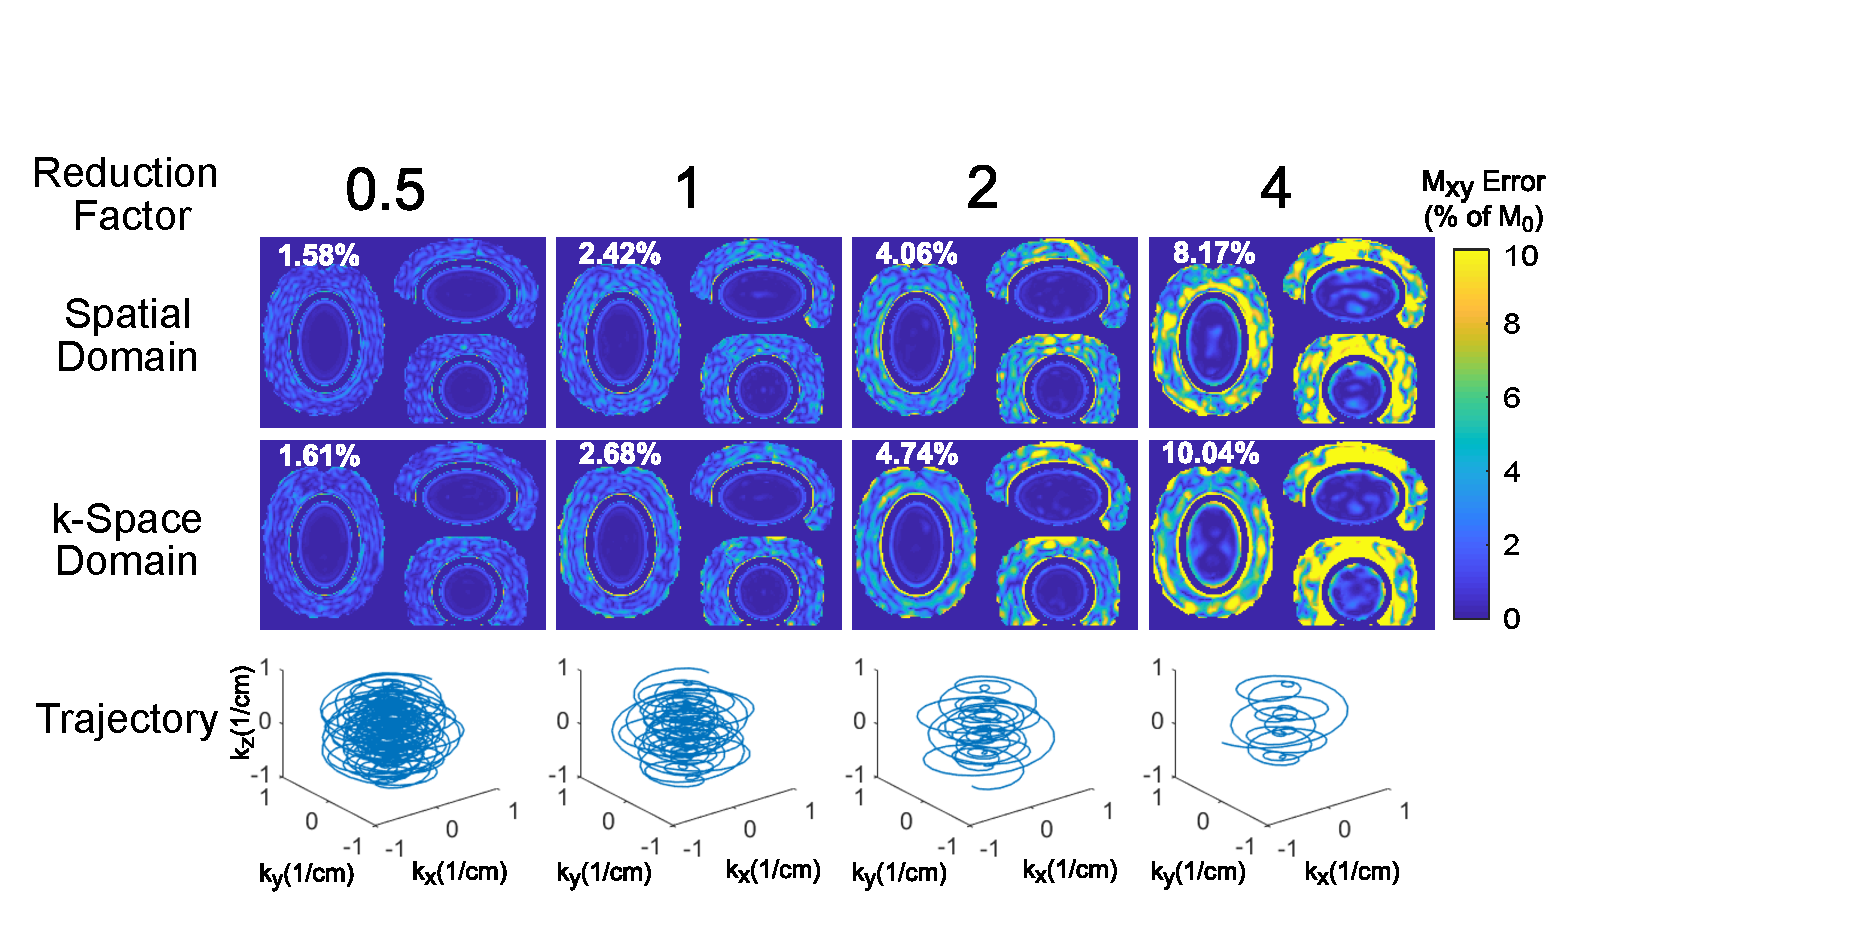
\includegraphics[width=\textwidth]{ReductionFactor}
	\caption{Normalized error maps and RMSEs for spatial domain design (first row) and k-space domain design (second row), 
	using excitation k-space trajectories with different reduction factors (third row).
	The reduction factors are referenced to the 10 ms trajectory in Figure \ref{fig:Target} (second column).}
	\label{fig:kspace_PTX_Acceleration}
\end{figure}


\begin{figure}
	\centering
	%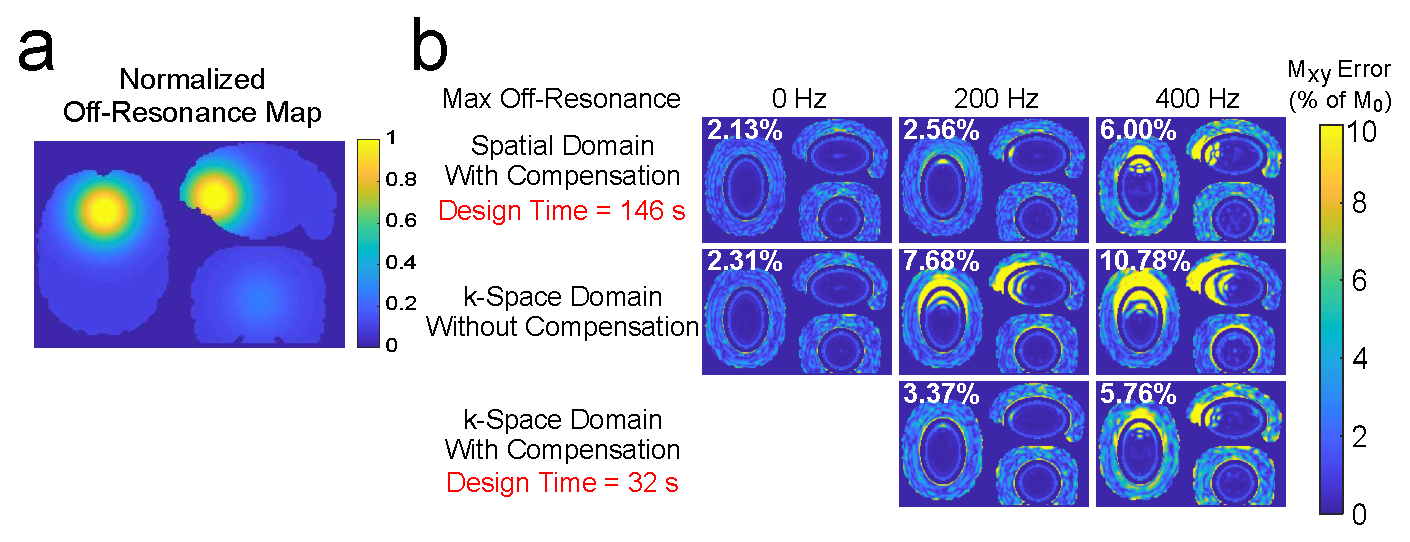
\includegraphics[width=\textwidth]{OffResonance}
	\caption{
	(a) Normalized off-resonance map containing a Gaussian distortion centered above the frontal sinus, 
	to mimic air-tissue susceptibility difference-induced $B_0$ inhomogeneity.
	(b) Normalized excitation maps and RMSEs for spatial domain design with off-resonance correction (first row), 
	and k-space domain design without and with off-resonance correction (second and third rows).}
	\label{fig:kspace_PTX_B0}
\end{figure}


\end{document}